
\documentclass[10pt]{report}
%Packages
\usepackage{multirow}
\usepackage{graphicx}
\usepackage[utf8]{inputenc}
\usepackage[T1]{fontenc}
\usepackage{aeguill}
\usepackage{amssymb}
\usepackage[french]{babel}
\usepackage{float}
\usepackage{fichetd}
\usepackage{mathenv}
\usepackage{tikz}
\usepackage[a4paper,pdftex=true]{geometry}
\usepackage{fancyvrb}

%Preamble

\input /Users/remy/cqls/texinputs/Cours/cqlsInclude
\input /Users/remy/cqls/texinputs/Cours/testInclude


\rightmargin -2cm
\leftmargin -1cm
\topmargin -2cm
\textheight 25cm

\newcommand{\redabr}{\textit{(rédaction abrégée) }}
\newcommand{\redstd}{\textit{(rédaction standard) }}

\setcounter{chapter}{5}
%Styles

%Title

\begin{document}




\appendix\chapter{Représentations\\graphiques~dans~l'A.E.P.}\label{TdAEPGraph}
\begin{IndicList}{Indications préliminaires} 
\item \textit{Objectif}~: Comme nous l'avons vu à la fiche T.D.~\ref{TdProb}, l'\textbf{A.E.P.} s'appuie sur l'étude descriptive de $m$ (grand) réalisations indépendantes $\Vect{y}_{[m]}:=\dataEmp[m]{y_{[\cdot]}}$ d'une variable aléatoire d'intérêt $Y$. Afin d'alléger l'introduction de l'\textbf{A.E.P.}, cette étude descriptive a été volontairement limitée à une étude quantitative n'utilisant aucune représentation graphique issue de la Statistique Descriptive. Les graphiques étant d'une grande aide pour représenter les répartitions de séries de données, ils vont donc nous aider à mieux appréhender le comportement aléatoire des variables aléatoires d'intérêt.
\item \textit{Représentations graphiques usuelles}~: Les représentations graphiques des répartitions diffèrent selon la nature des variables. Ainsi, lorsque la variable est de nature discrète (i.e. les modalités ou valeurs possibles sont dénombrables), on utilise un diagramme en bâton, et lorsqu'elle est de nature continue (i.e. à valeurs dans un continuum qui est non dénombrable), un histogramme est utilisé. Ce choix pose problème lorsqu'une étude expérimentale nous amène à comparer sur un même graphique des répartitions de plusieurs variables n'ayant pas la même nature. Il n'est pas possible de représenter une variable continue par un diagramme en bâton mais il en est tout autrement pour une variable discrète qui peut se représenter via un \underline{histogramme discret} que nous allons introduire très prochainement. 
\item \textit{Histogramme (continu)}~: Rappelons les règles générales pour construire un histogramme représentant la répartition de la série  $z_1,z_2,\cdots,z_m$~:
\begin{enumerate}
\item L'ensemble des modalités est découpé en une partition d'intervalles pas forcément de même largeur.
\item Chaque intervalle de la partition est représenté par un rectangle ayant pour base l'intervalle et de surface égale à la proportion des $z_1,z_2,\cdots,z_m$ appartenant au dit intervalle.
\item La somme de tous les rectangles est donc égale à 100\%=1.
\end{enumerate}
Pour construire pratiquement un histogramme, il est conseillé au préalable de trier les $z_1,z_2,\cdots,z_m$ afin de les regrouper et ainsi de les affecter  plus facilement à leurs intervalles d'appartenance. Au lieu de directement construire les rectangles associés aux intervalles de la partition, nous avons choisi d'associer à chaque donnée $z_i$ un i\ieme\ rectangle, que l'on appellera \underline{brique} (l'histogramme étant un vu  de manière imagée comme un ``mur")~:
\begin{enumerate}
\item Toute brique associée à $z_i$ a pour base l'intervalle d'appartenance de $z_i$ et a une surface égale à $\frac1m$.
\item La somme de toutes les briques associées aux $z_1,z_2,\cdots,z_m$ est donc égale à 1.
\item Un rectangle associé à un intervalle est l'empilement de toutes les briques associés aux $z_i$ de l'intervalle.  
\end{enumerate}
Cette version de l'histogramme est équivalente à la version originale et propose en plus une représentation individualisée de toutes les données $z_1,z_2,\cdots,z_m$. Ce point particulier sera un atout pour comprendre la représentation graphique usuelle de loi de probabilités de variable aléatoire continue. 
\item \textit{Histogramme discret}~: Dans le même esprit, nous allons maintenant présenter la notion d'\underline{histogramme discret} en l'adaptant à des données $z_1,z_2,\cdots,z_m$ à valeurs dans un espace dénombrable (donc pas dans un continuum)~:
\begin{enumerate}
\item Une brique associée à $z_i$ a pour surface $\frac1m$ et sa base est centrée en $z_i$ (à la différence d'une brique d'un histogramme continu où $z_i$ doit appartenir à l'intervalle représentant la base de la brique).
\item Les bases des briques sont fixées de sorte que le mur (i.e. l'histogramme) constitué de l'ensemble des briques ait le moins d'espace (trou) possible. Les briques voisines doivent se toucher dès que possible.
\item La somme des briques est toujours égale à 100\%=1 et l'empilement des briques associées aux données ayant même modalité forme un rectangle dont la surface est égale à la proportion des données égales à la modalité associée.  
\end{enumerate}
\textbf{IMPORTANT}~: Nous remarquons que dans la représentation d'histogramme (discret ou continu) les valeurs en ordonnée n'ont pas d'unité réellement interprétable. En revanche, lorsque les bases des rectangles sont toutes les mêmes, les hauteurs pourront donc être comparées entre elles pour nous éclairer sur la répartition des données puisque les aires des surfaces des rectangles (vues comme des empilements de briques) représentent naturellement des proportions de données.  
\end{IndicList}


\begin{exercice}[Histogramme continu] ${ }$\label{ex:histMoyUnifs}
Cet exercice fait suite à l'exercice~\ref{ex:sommeUnifs} mais dans l'esprit de l'exercice~\ref{ex:loiMoyenne} puisqu'on s'intéresse à la moyenne plutôt que la somme. Voici 4 graphiques représentant les histogrammes continus des $m=200$, 2000, 5000, 10000 premières réalisations de la variable $M_2:=\frac{Y_1+Y_2}2=\frac{S}2$. Nous rappelons que les $m=10000$ réalisations de $S$ avaient été stockées dans le vecteur \texttt{s} en \texttt{R}. Les $m=10000$ réalisations $\dataEmp[m]{m_{2,[\cdot]}}$ de $M_2$ sont donc accessibles en \texttt{R} via l'instruction \texttt{s/2}. 







\centerline{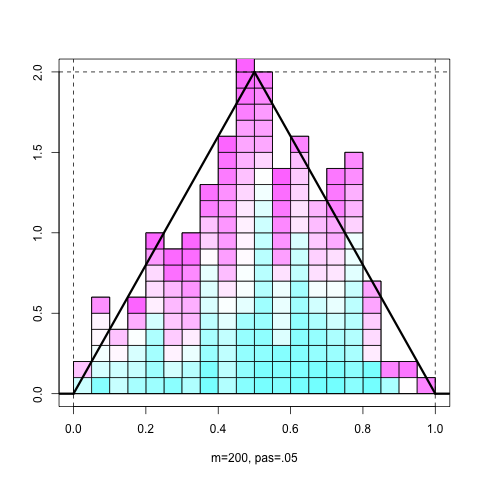
\includegraphics[width=8cm,height=8cm]{img/deuxUnif200} 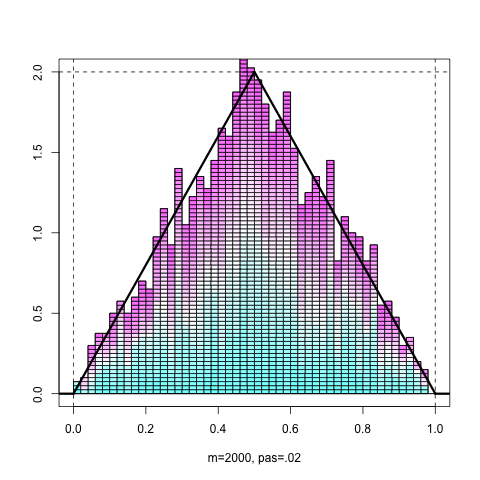
\includegraphics[width=8cm,height=8cm]{img/deuxUnif2000}}
\centerline{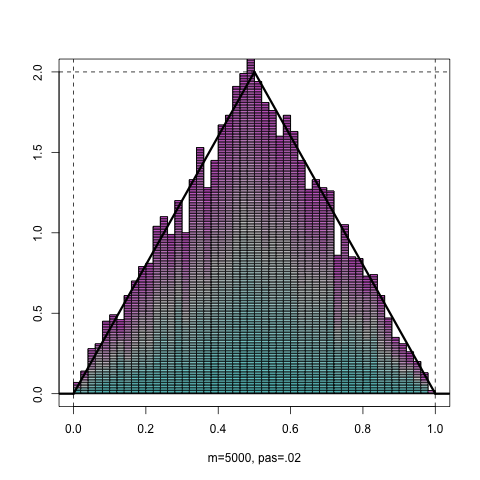
\includegraphics[width=8cm,height=8cm]{img/deuxUnif5000} 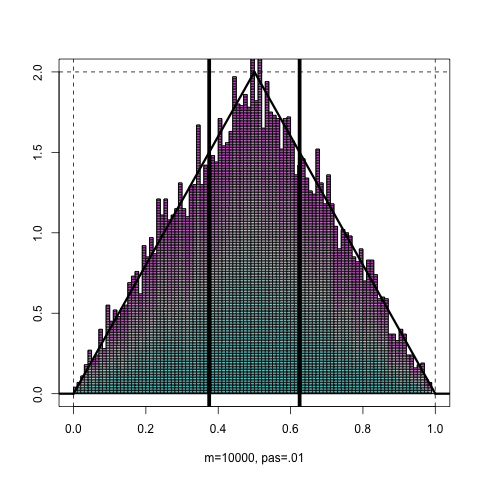
\includegraphics[width=8cm,height=8cm]{img/deuxUnif10000}}
Dans le contexte de l'\textbf{A.E.P.}, les intervalles d'un histogramme continu peuvent sans restriction être de même largeur (car $m$ est censé être suffisamment grand). 
Le ``pas" d'un histogramme nomme en général la largeur du plus petit de ces intervalles.
\begin{enumerate}
\item Pour chaque graphique, indiquez quelle est la surface d'une brique.  
\item Lequel de ces graphiques est le plus informatif~? A partir de ce dernier, êtes-vous en mesure de déterminer les valeurs de $M_2$ qui sont les plus probables~?
\item  Identifiez les briques associées aux valeurs comprises entre $\frac38$ et $\frac58$ incluses. Quelle est la valeur de l'aire de la surface occupée par ces briques en vous rappelant que la proportion des $\dataEmp[m]{m_{2,[\cdot]}}$ comprises entre $\frac38$ et $\frac58$  est fourni par~:\\
\begin{Verbatim}[frame=leftline,fontfamily=tt,fontshape=n,numbers=left]
> mean(3/8<=s/2 &  s/2<=5/8)
[1] 0.4262
\end{Verbatim}

\item Sauriez-vous alors évaluer approximativement la probabilité $\PPP{M_2\in [\frac38,\frac58]}$~?
\item Est-il possible d'évaluer approximativement $\PPP{M_2=\frac12}$ qui via l'\textbf{A.E.P.} est approchée grâce à~:
\begin{Verbatim}[frame=leftline,fontfamily=tt,fontshape=n,numbers=left]
> mean(s/2==1/2)
[1] 0
\end{Verbatim}

Que faudrait-il faire pour pouvoir y arriver~?
\item En s'imaginant que le pas $\to0$ au fur et à mesure que $m\to+\infty$, pouvez-vous décrire à quoi ressemblera une brique~? Même question pour le mur de briques~? Représentez-le sur le graphique en ne dessinant que le ``dessus" (i.e. contour supérieur) du mur. Vu comme une fonction, comment interprèteriez-vous le contour supérieur du mur~?  

\item Un mathématicien, sollicité pour nous assister dans l'étude de l'\textbf{A.M.P.}, nous apprend qu'il est classique de caractériser le comportement aléatoire de $M_2$ en fournissant la densité de probabilité (qui porte bien son nom!) s'exprimant ici mathématiquement par~:
\[
f_{M_2}(t)=\left\{\begin{array}{ll}
4t & \mbox{si }t\in [0,\frac12]\\
4-4t & \mbox{si }t\in [\frac12,1]\\
0 & \mbox{sinon}
\end{array}\right.
\]
Représentez cette fonction sur le dernier graphique et comparez-la avec les histogrammes continus. Sont-ils très différents de la fonction~?
\item Le mathématicien nous annonce que  $\PPP{M_2\in [\frac38,\frac58]}=\displaystyle\int_{\frac38}^{\frac58} f_{M_2}(t)dt$ qui est représentée graphiquement par la surface des points sous la courbe $f_{M_2}(t)$ et dont les abscisses sont compris entre $\frac38$ et $\frac58$. Représentez alors $\PPP{M_2\in [\frac38,\frac58]}$ sur le graphique. Cela ne vous rappelle pas quelquechose~?
Sachant qu'il n'est pas difficile de montrer que $\PPP{M_2\in [\frac38,\frac58]}=\PPP{S\in [\frac34,\frac54]}=\frac7{16}\simeq 43.75\%$ (déjà évaluée à l'exercice~\ref{ex:sommeUnifs}), évaluez l'aire de la surface représentant cette probabilité. 
\item Quelle est la valeur exacte de $\PPP{M_2=\frac12}$~?
\item Sélectionnez la bonne réponse parmi les réponses (proposées en suivant entre parenthèses)~:\\
La modalité $\frac12$ est le mode de la loi de $M_2$ car $\frac12$ est la valeur qui maximise la fonction \underline{\hspace*{1cm}} ( $\mathbf{p_{M_2}(x)}:=\PPP{M_2=x}$ ou $\mathbf{f_{M_2}(x)}$ ou $\mathbf{F_{M_2}(x)}:=\PPP{M_2\leq x}$ ).
Cela se traduit littéralement par~: $\frac12$ est la valeur de plus grande \underline{\hspace*{2cm}}( \textbf{probabilité} ou \textbf{densité de probabilité} ou \textbf{fonction de répartition} ).

\begin{Indication}{A retenir}
$\to$ La \underline{densité de probabilité} caractérisant la loi de probabilité d'une v.a. continue $Y$ est vue via l'\textbf{A.E.P.} comme le \texttt{contour supérieur} de \textbf{l'histogramme à ``pas zéro" d'une infinité de ses réalisations} (i.e. $\Vect{y}_{[+\infty]}:=\dataEmp[+\infty]{y_{[\cdot]}}$). De manière plus imagée, cet histogramme se décrit comme \textbf{un mur de briques devenues points}  ou comme \textbf{un ``tas de points"} (pour traduire la notion d'empilement) où chaque point est associé à une des réalisations. Autrement dit, tous ces objets permettent de décrire de manière très synthétique l'ensemble de ``tous" les résultats possibles (représentés par les composantes de $\Vect{y}_{[+\infty]}$) de la variable aléatoire $Y$.\\ 
\noindent $\to$ La probabilité $\PPP{Y\in [a,b]}=\displaystyle\int_a^b f_{Y}(t)dt$ dans le contexte de l'\textbf{A.M.P.} correspond via l'\textbf{A.E.P.} à la proportion des composantes de $\Vect{y}_{[+\infty]}$ appartenant à $[a,b]$. Du points de vue de l'\textbf{A.M.P.} ou de celui de l'\textbf{A.E.P.}, elle se représente par la surface occupée par les points sous la courbe $f_Y$ et d'abscisses appartenant à $[a,b]$.  
\end{Indication}

\end{enumerate}
\end{exercice}
\begin{exercice}[Histogramme discret] ${ }$\label{ex:histMoyDes}
On s'intéresse à la loi de probabilité de la moyenne $M_2:=\frac{Y_1+Y_2}2=\frac{S}2$ où $S$ représente la somme de deux dés (introduite auparavant à l'exercice~\ref{ex:sommeDes}). Le but est ici d'introduire la notion d'histogramme discret qui n'est pas la représentation graphique la plus usuelle pour représenter une variable aléatoire discrète. Voici 4 histogrammes discrets pour les $m=200$, 1000, 2000 et 5000 premières somme des deux dés. Remarquons que dans le cadre de l'exercice, nous aurions pu nous limiter à la représentation graphique usuelle en diagramme en bâton
puisque nous n'aurons aucune intention de comparer la loi de probabilité de $M_2$ avec celle d'une loi de probabilité associée à une variable aléatoire continue. Ce sera en revanche le cas dans l'exercice~\ref{ex:histMoyenne}.
    








Afin de mettre en avant les caractéristiques les distinguant des histogrammes continus, nous avons complété les histogrammes en identifiant les modalités de $M_2$ par des petits traits en gras sur l'axe des abscisses prolongés par des lignes verticales en trait pointillé.

\centerline{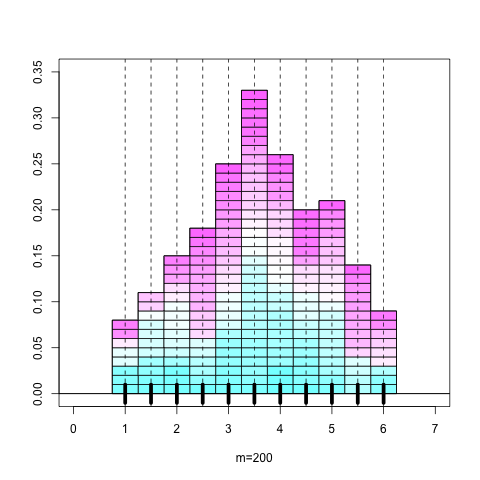
\includegraphics[width=8cm,height=8cm]{img/deuxDes200} 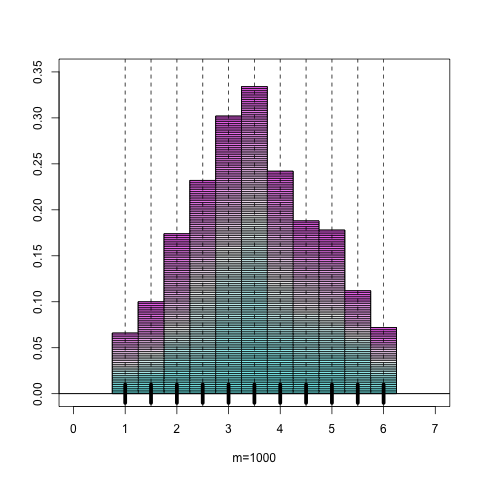
\includegraphics[width=8cm,height=8cm]{img/deuxDes1000}}
\centerline{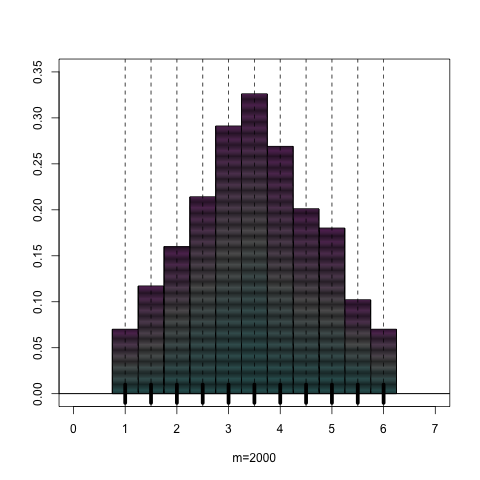
\includegraphics[width=8cm,height=8cm]{img/deuxDes2000} 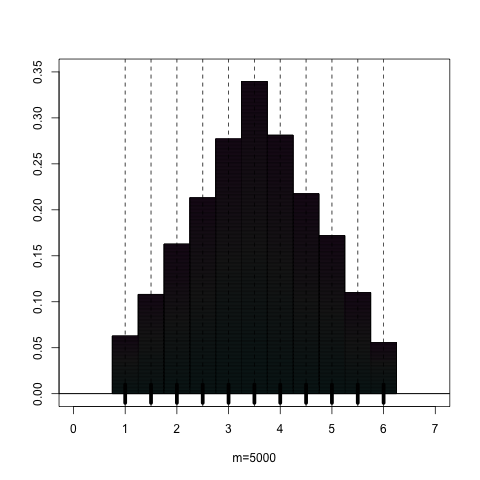
\includegraphics[width=8cm,height=8cm]{img/deuxDes5000}}


\begin{enumerate}
\item Quelles sont les largeurs des briques utilisées dans ces histogrammes discrets~? Changent-elles lorsque $m$ augmente (justifier votre réponse)~? Sur chacun des graphiques, indiquez l'aire de la surface de chaque brique. 
\item A partir du premier graphique, donnez un ordre de grandeur de la probabilité $\PPP{M_2=1}$. Quelle est l'aire de la surface occupée par les briques associées aux $m_{2,[k]}=1$~? A-t'on vraiment besoin de voir les briques individuellement pour évaluer $\PPP{M_2=1}$~? Si vous avez répondu non, appliquez cela sur le dernier graphique puisque les briques ne sont pas distinguables individuellement tellement elles sont plates.
\item Le graphique suivant fournit deux histogrammes discrets l'un correspondant à $m=5000$ et l'autre à celui $m\to+\infty$. Deux types de trait (simple et en gras) ont été utilisés pour les représenter. Sauriez-vous les identifier~? Evaluez (le plus précisément possible) $\PPP{M_2=1}$ ainsi que $\PPP{M_2\in\{1,1.5,6\}}$.
      

\centerline{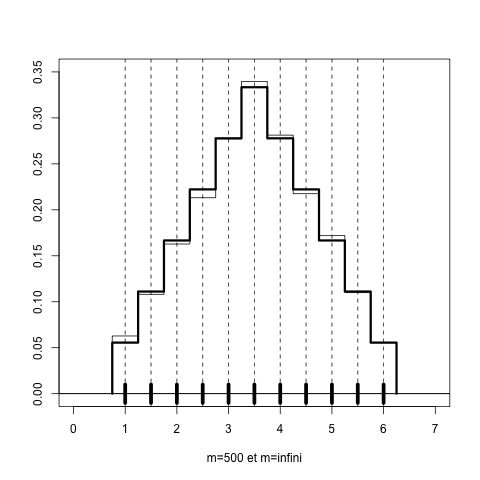
\includegraphics[width=8cm,height=8cm]{img/deuxDesInf}}
\end{enumerate}
\end{exercice}
\begin{Indication}{A retenir}
\noindent $\to$ L'histogramme discret s'interprète de la même manière qu'un histogramme continu où les probabilités (ou proportions) sont mesurées via des aires de surfaces.\\
\noindent $\to$ A la différence d'un histogramme continu, dans un histogramme discret~:
\begin{itemize} 
\item les briques sont de largeur fixe (même lorsque $m$ varie)
\item la base d'une brique n'a pas vraiment de sens
\item seul le centre de la base d'une brique a un sens puisqu'il indique la valeur associée qui se lit en abscisse (surtout si la brique n'est pas la première à avoir été empilée).  
\end{itemize} 
\end{Indication}
\begin{exercice}[Histogramme de moyenne] ${ }$ \label{ex:histMoyenne}
L'étude menée est la suite de l'exercice~\ref{ex:loiMoyenne}. Ayant introduit les notions d'histogrammes discret et continu, nous allons pouvoir apprécier de visualiser le théorème de la limite centrale notamment dans le cadre de l'exemple de la moyenne de dés. Voici pour commencer, 2 graphiques représentant les contours supérieurs des histogrammes (discrets pour l'exemple du dé à gauche et continu pour l'exemple de la loi uniforme sur $[1,6]$ à droite) des lois de probabilité $M_n$ pour $n=1,2,4,16,64$. Les échelles sont identiques pour les 2 graphiques.














































\centerline{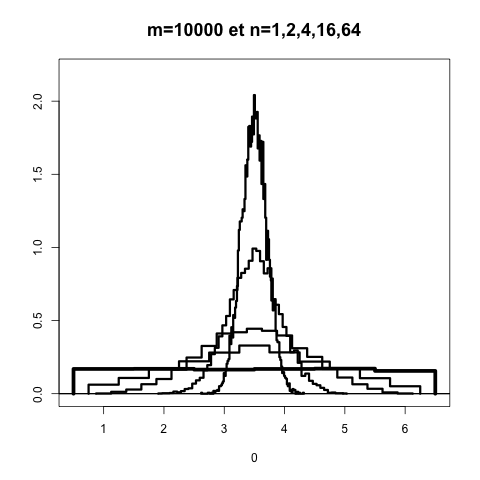
\includegraphics[width=8cm,height=8cm]{img/moyDes}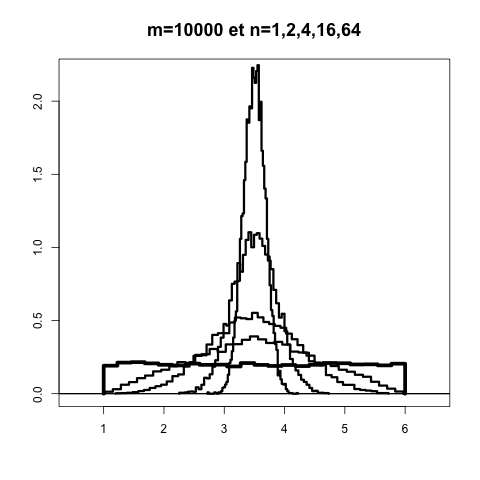
\includegraphics[width=8cm,height=8cm]{img/moyUnifs}}

\begin{enumerate}
\item Pour chaque graphique, quelle est l'histogramme qui représente via l'\textbf{A.E.P.} la loi de probabilité approximative de $Y_1$~? 
\item Ces représentations graphiques expriment-elles le résultat que nous avions décrit sur le procédé de moyennisation qui concentre les modalités~?
\item Comparez les 2 graphiques. Pour quelle étude (dé ou uniforme), la moyenne est de plus grande variance~?
\item Sauriez-vous anticiper les histogrammes pour le cas où $n\to+\infty$ avec $m\to+\infty$~?
\item Comme il n'est pas possible d'observer la forme de l'histogramme dans le cas précédent, il est naturel de faire comme un photographe en rezoomant le graphique de sorte à pouvoir mieux cadrer l'histogramme sur le graphique. C'est aussi ce que fait automatiquement le logiciel~\texttt{R} comme on peut le voir dans la série de graphiques suivants~:\\[0.25cm]
\hspace*{-2.3cm}\begin{tabular}{|c|c|c|c|}\hline
\multicolumn{2}{|c|}{Exemple du dé: $Y_i\leadsto \mathcal{U}(\{1,2,3,4,5,6\})$} & \multicolumn{2}{c|}{Exemple de l'uniforme: $Y_i\leadsto \mathcal{U}([1,6])$}\\\hline
loi de $M_n$ & loi de $\Delta_n$ & loi de $M_n$ & loi de $\Delta_n$\\\hline
%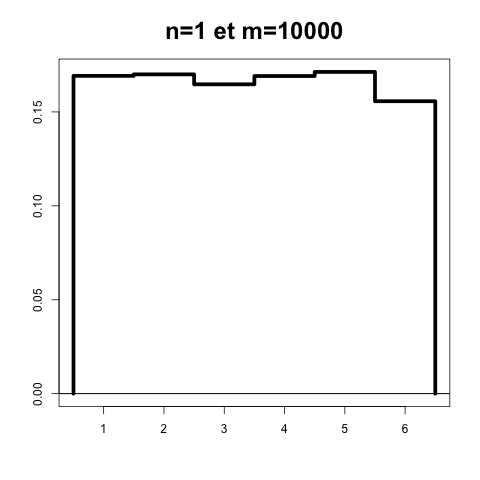
\includegraphics[width=4cm,height=4cm]{img/n1MoyDes} & 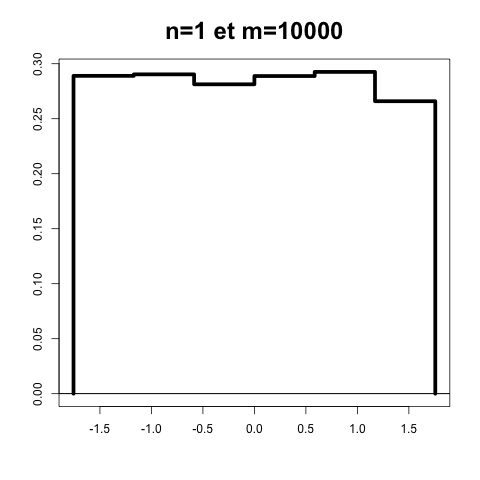
\includegraphics[width=4cm,height=4cm]{img/n1DeltaMoyDes} & 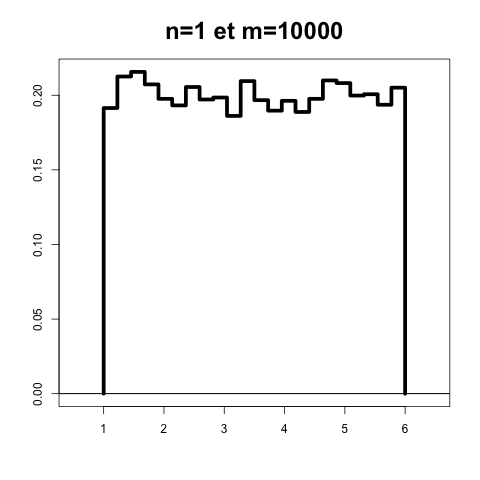
\includegraphics[width=4cm,height=4cm]{img/n1MoyUnifs} & 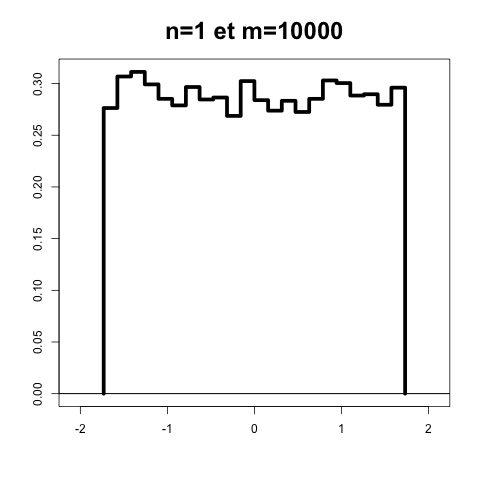
\includegraphics[width=4cm,height=4cm]{img/n1DeltaMoyUnifs}\\\hline
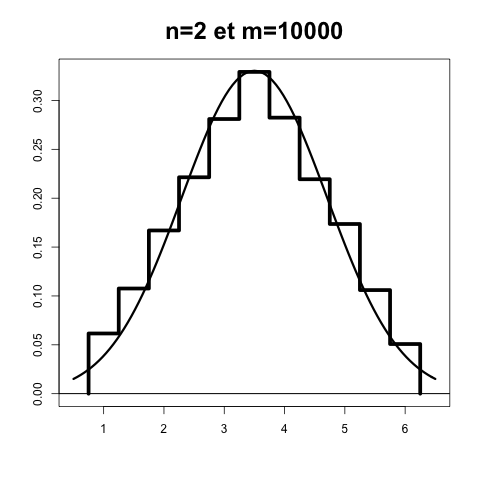
\includegraphics[width=4cm,height=4cm]{img/n2MoyDes} & 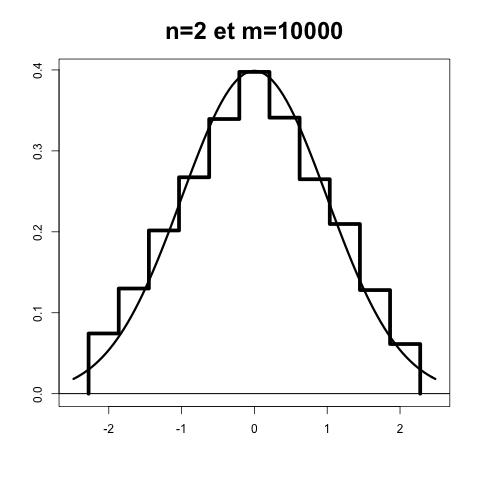
\includegraphics[width=4cm,height=4cm]{img/n2DeltaMoyDes} & 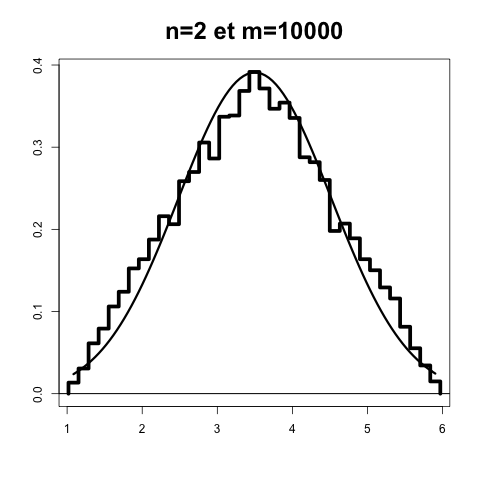
\includegraphics[width=4cm,height=4cm]{img/n2MoyUnifs} & 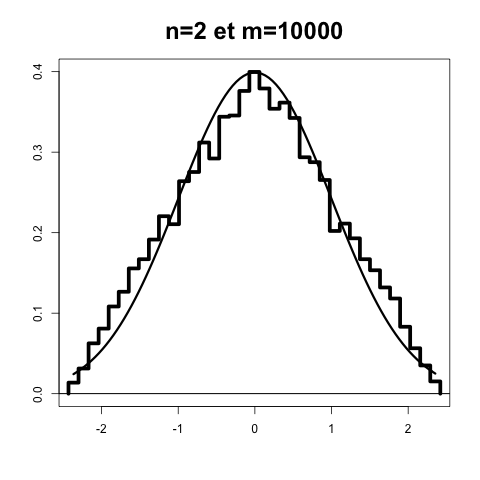
\includegraphics[width=4cm,height=4cm]{img/n2DeltaMoyUnifs}\\\hline
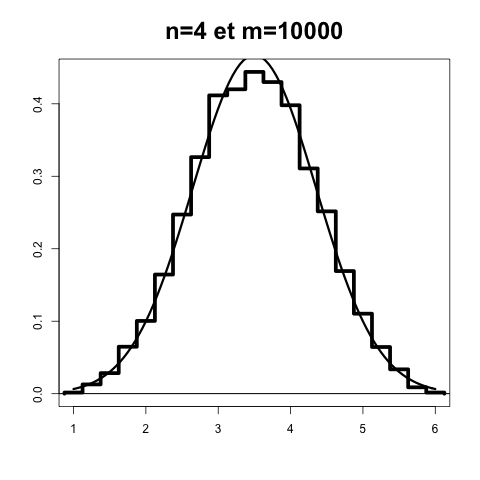
\includegraphics[width=4cm,height=4cm]{img/n4MoyDes} & 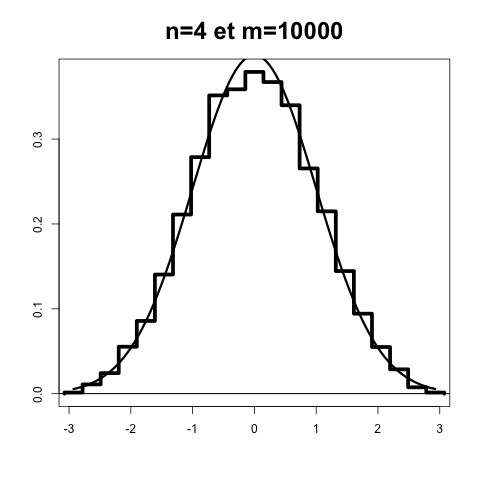
\includegraphics[width=4cm,height=4cm]{img/n4DeltaMoyDes} & 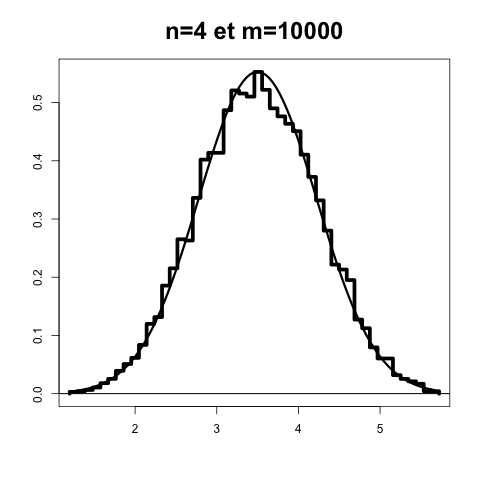
\includegraphics[width=4cm,height=4cm]{img/n4MoyUnifs} & 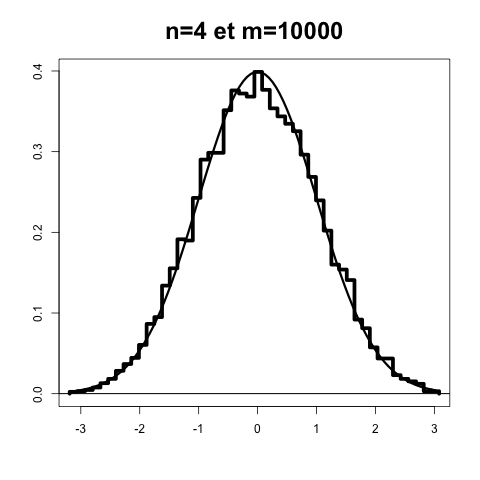
\includegraphics[width=4cm,height=4cm]{img/n4DeltaMoyUnifs}\\\hline
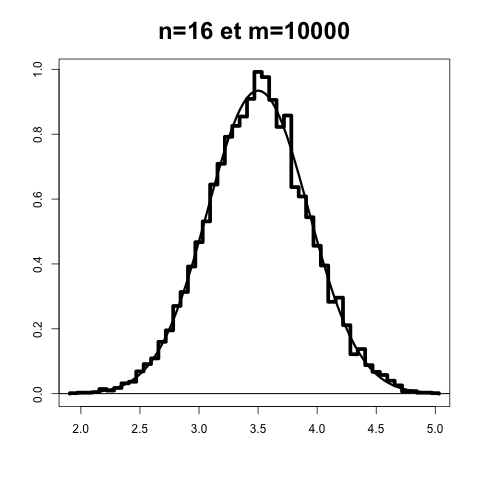
\includegraphics[width=4cm,height=4cm]{img/n16MoyDes} & 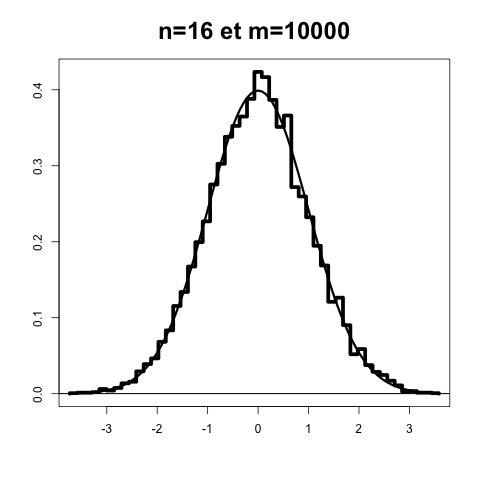
\includegraphics[width=4cm,height=4cm]{img/n16DeltaMoyDes} & 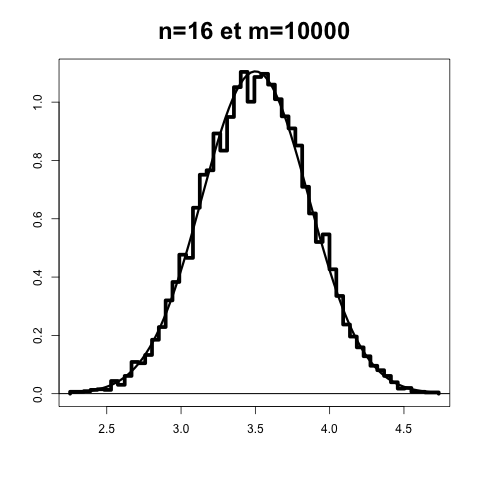
\includegraphics[width=4cm,height=4cm]{img/n16MoyUnifs} & 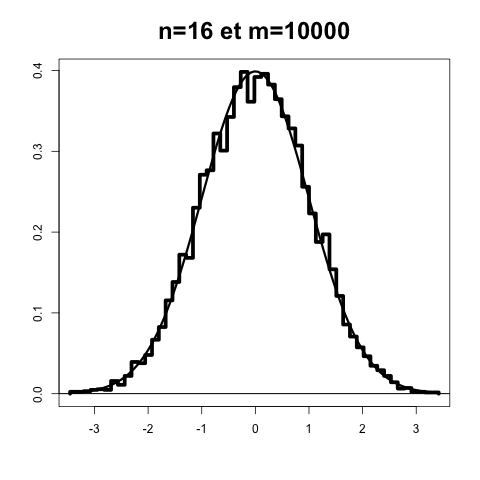
\includegraphics[width=4cm,height=4cm]{img/n16DeltaMoyUnifs}\\\hline
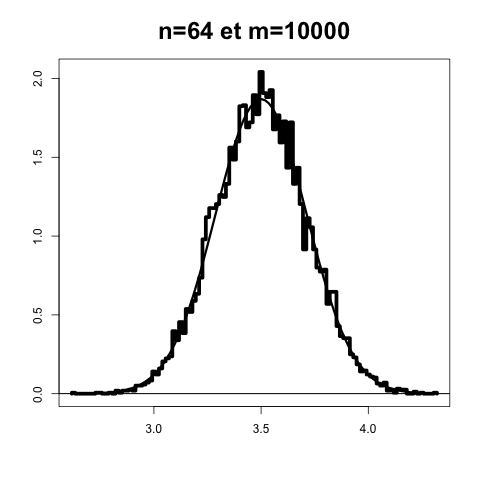
\includegraphics[width=4cm,height=4cm]{img/n64MoyDes} & 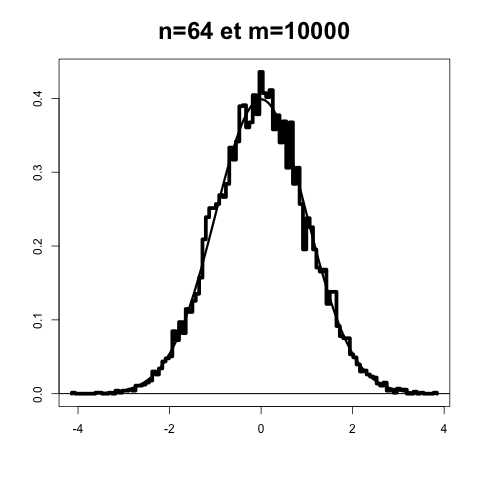
\includegraphics[width=4cm,height=4cm]{img/n64DeltaMoyDes} & 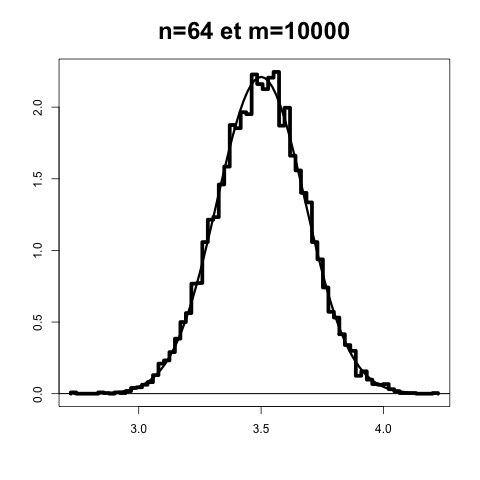
\includegraphics[width=4cm,height=4cm]{img/n64MoyUnifs} & 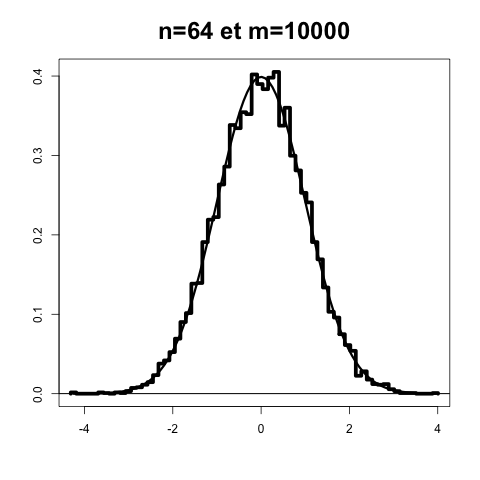
\includegraphics[width=4cm,height=4cm]{img/n64DeltaMoyUnifs}\\\hline
\end{tabular}
\item Pour les 2 exemples et pour chaque $n$, comparez la forme de l'histogramme (en trait le plus épais) des réalisations de $M_n$ avec celle de l'histogramme (en trait le plus épais) des réalisations $\Delta_n$~? Expliquez pourquoi il en est ainsi~?
\item Pourquoi ces histogrammes sont-ils de plus en plus irréguliers lorsque $n$ augmente~? Qu'aurait dû faire l'expérimentateur pour qu'il n'en soit pas ainsi~? Pouvez-vous tout de même imaginer ce qui ce serait passé lorsque $m\to+\infty$~?
\item D'après le Théorème de la limite centrale, on peut mathématiquement affirmer, lorsque $n$ est suffisamment grand (convention simplifiée appliquée dans ce cours: $n\geq 30$)~:
\[
  M_n\SuitApprox \mathcal{N}\left(\EEE{Y_1},\sqrt{\frac{\VVV{Y_1}}{n}}\right) \Leftrightarrow \Delta_n:=\frac{M_n-\EEE{Y_1}}{\sqrt{\frac{\VVV{Y_1}}{n}}} \SuitApprox \mathcal{N}(0,1).
\]
Aussi, on rappelle que, pour l'exemple du dé, $\VVV{Y_1}=2.9167$ et que, pour l'exemple de la loi uniforme sur $[1,6]$,  $\VVV{Y_1}=\frac{25}{12}$.\\
Pour chaque graphique, que représente la courbe en trait le plus fin~?  Est-elle de plus en plus ressemblante à l'histogramme en trait le plus épais lorsque $n$ augmente (Indication~: éviter de tenir compte du caractère irrégulier de l'histogramme quand $n$ augmente uniquement dû au fait que $m$ aurait dû être augmenté en même temps que $n$)~?
\item Dans le contexte de l'\textbf{A.E.P.}, comment décririez-vous ces courbes~? %répartitions de m=+\infty de \mathcal{N}\left(\EEE{Y_1},\sqrt{\frac{\VVV{Y_1}}{n}}\right)
Dans l'exemple du dé, les deux histogrammes représentées sur chaque graphique sont-ils de la même nature~? Avez-vous une idée sur comment illustrer graphiquement le Théorème de la limite centrale sans l'utilisation de l'histogramme discret (\textit{Indication}~: Une réponse très courte est bien venue)~?  
\item Le Théorème de la limite centrale s'appliquant pour tout $Y_1$ ayant n'importe quelle loi de probabilité admettant une moyenne et une variance finies, imaginez la même série de graphiques que précédemment mais pour d'autres exemples que ceux (uniformes) choisis dans cette étude.   
\end{enumerate}

\end{exercice}






\end{document}


